\providecommand{\main}{../../../..}
\documentclass[\main/dresen_thesis.tex]{subfiles}

\begin{document}
  \label{sec:looselyPackedNS:nanoparticle:tem}
  \begin{figure}[!htbp]
    \centering
    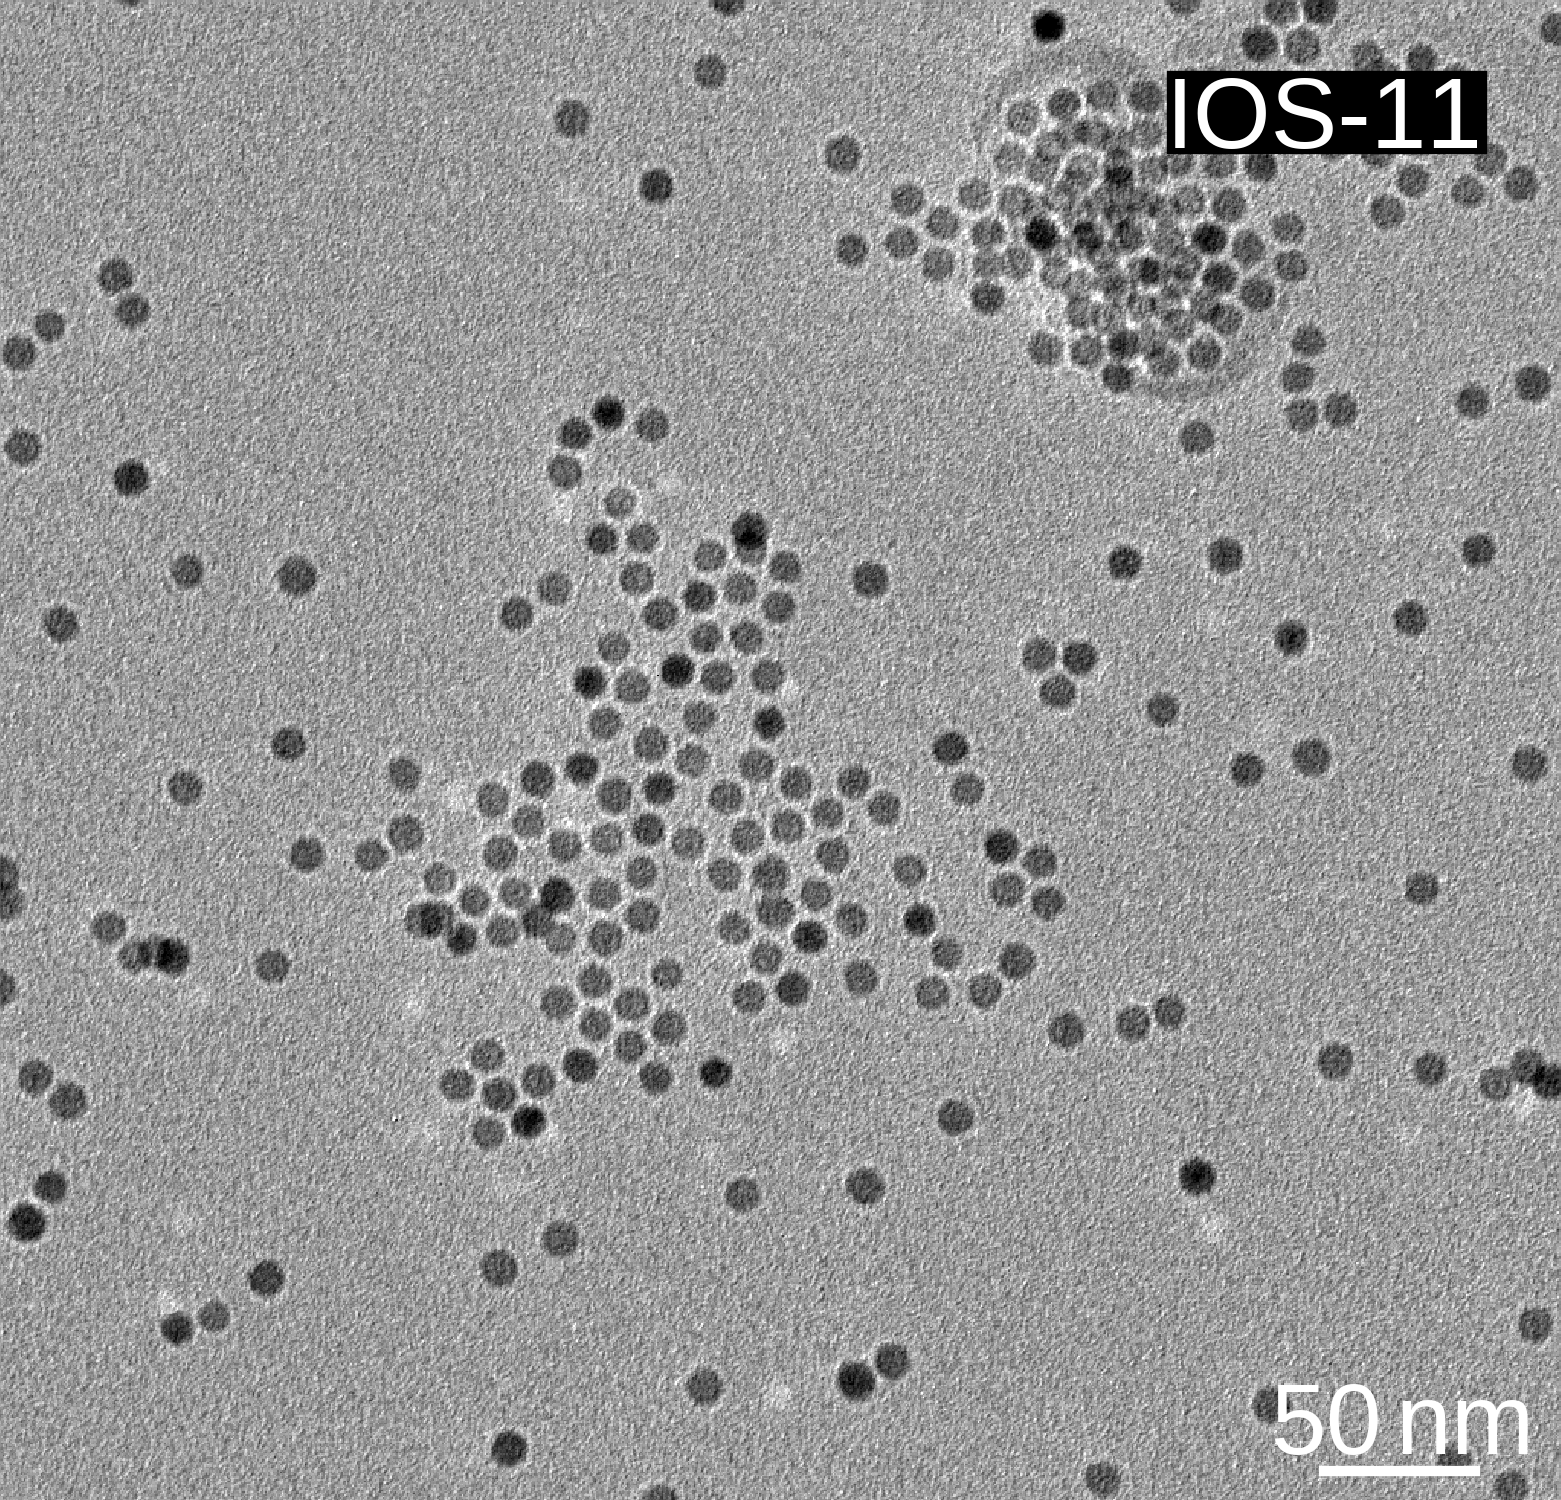
\includegraphics{looselyPackedNP_TEM_PMK18}
    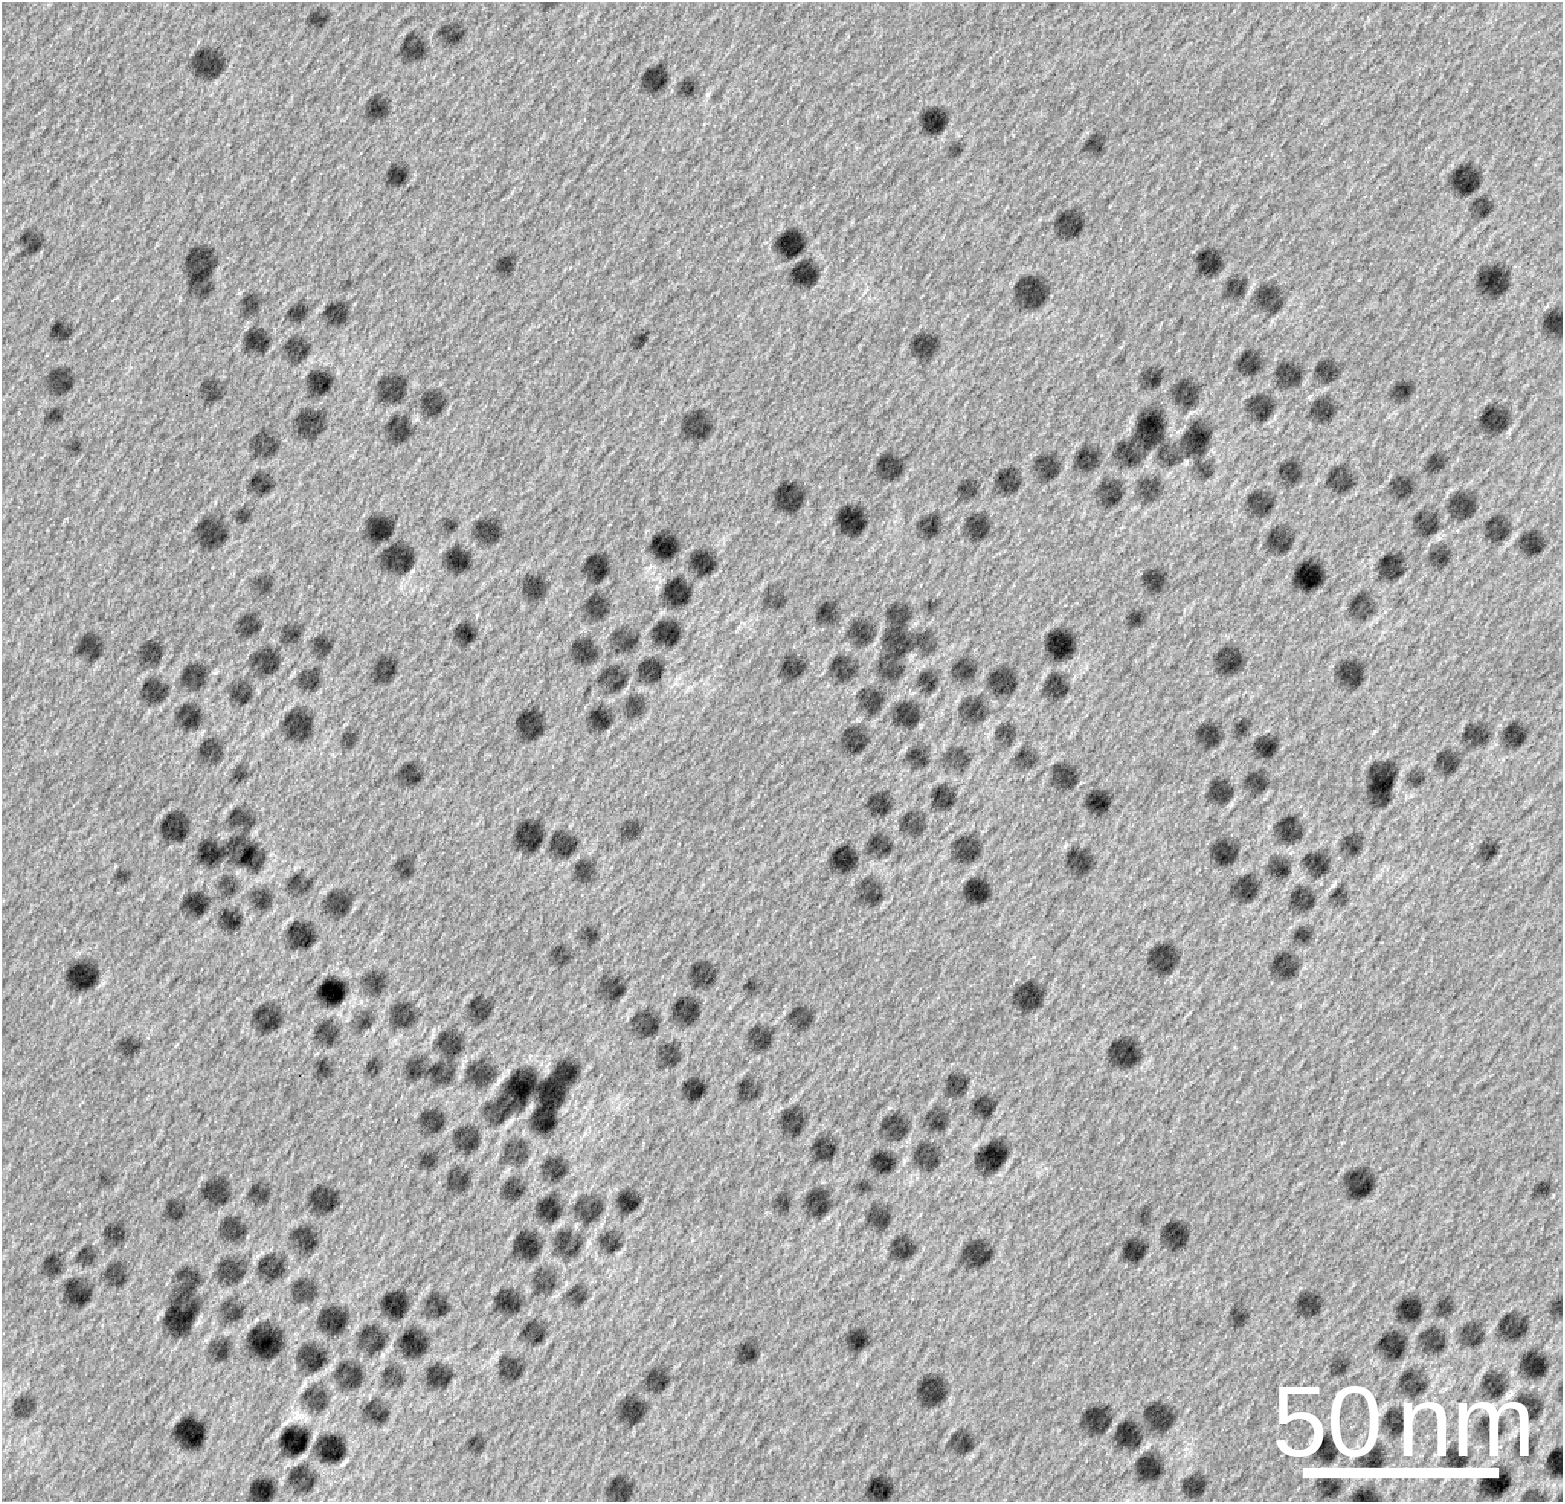
\includegraphics{looselyPackedNP_TEM_KWi338}
    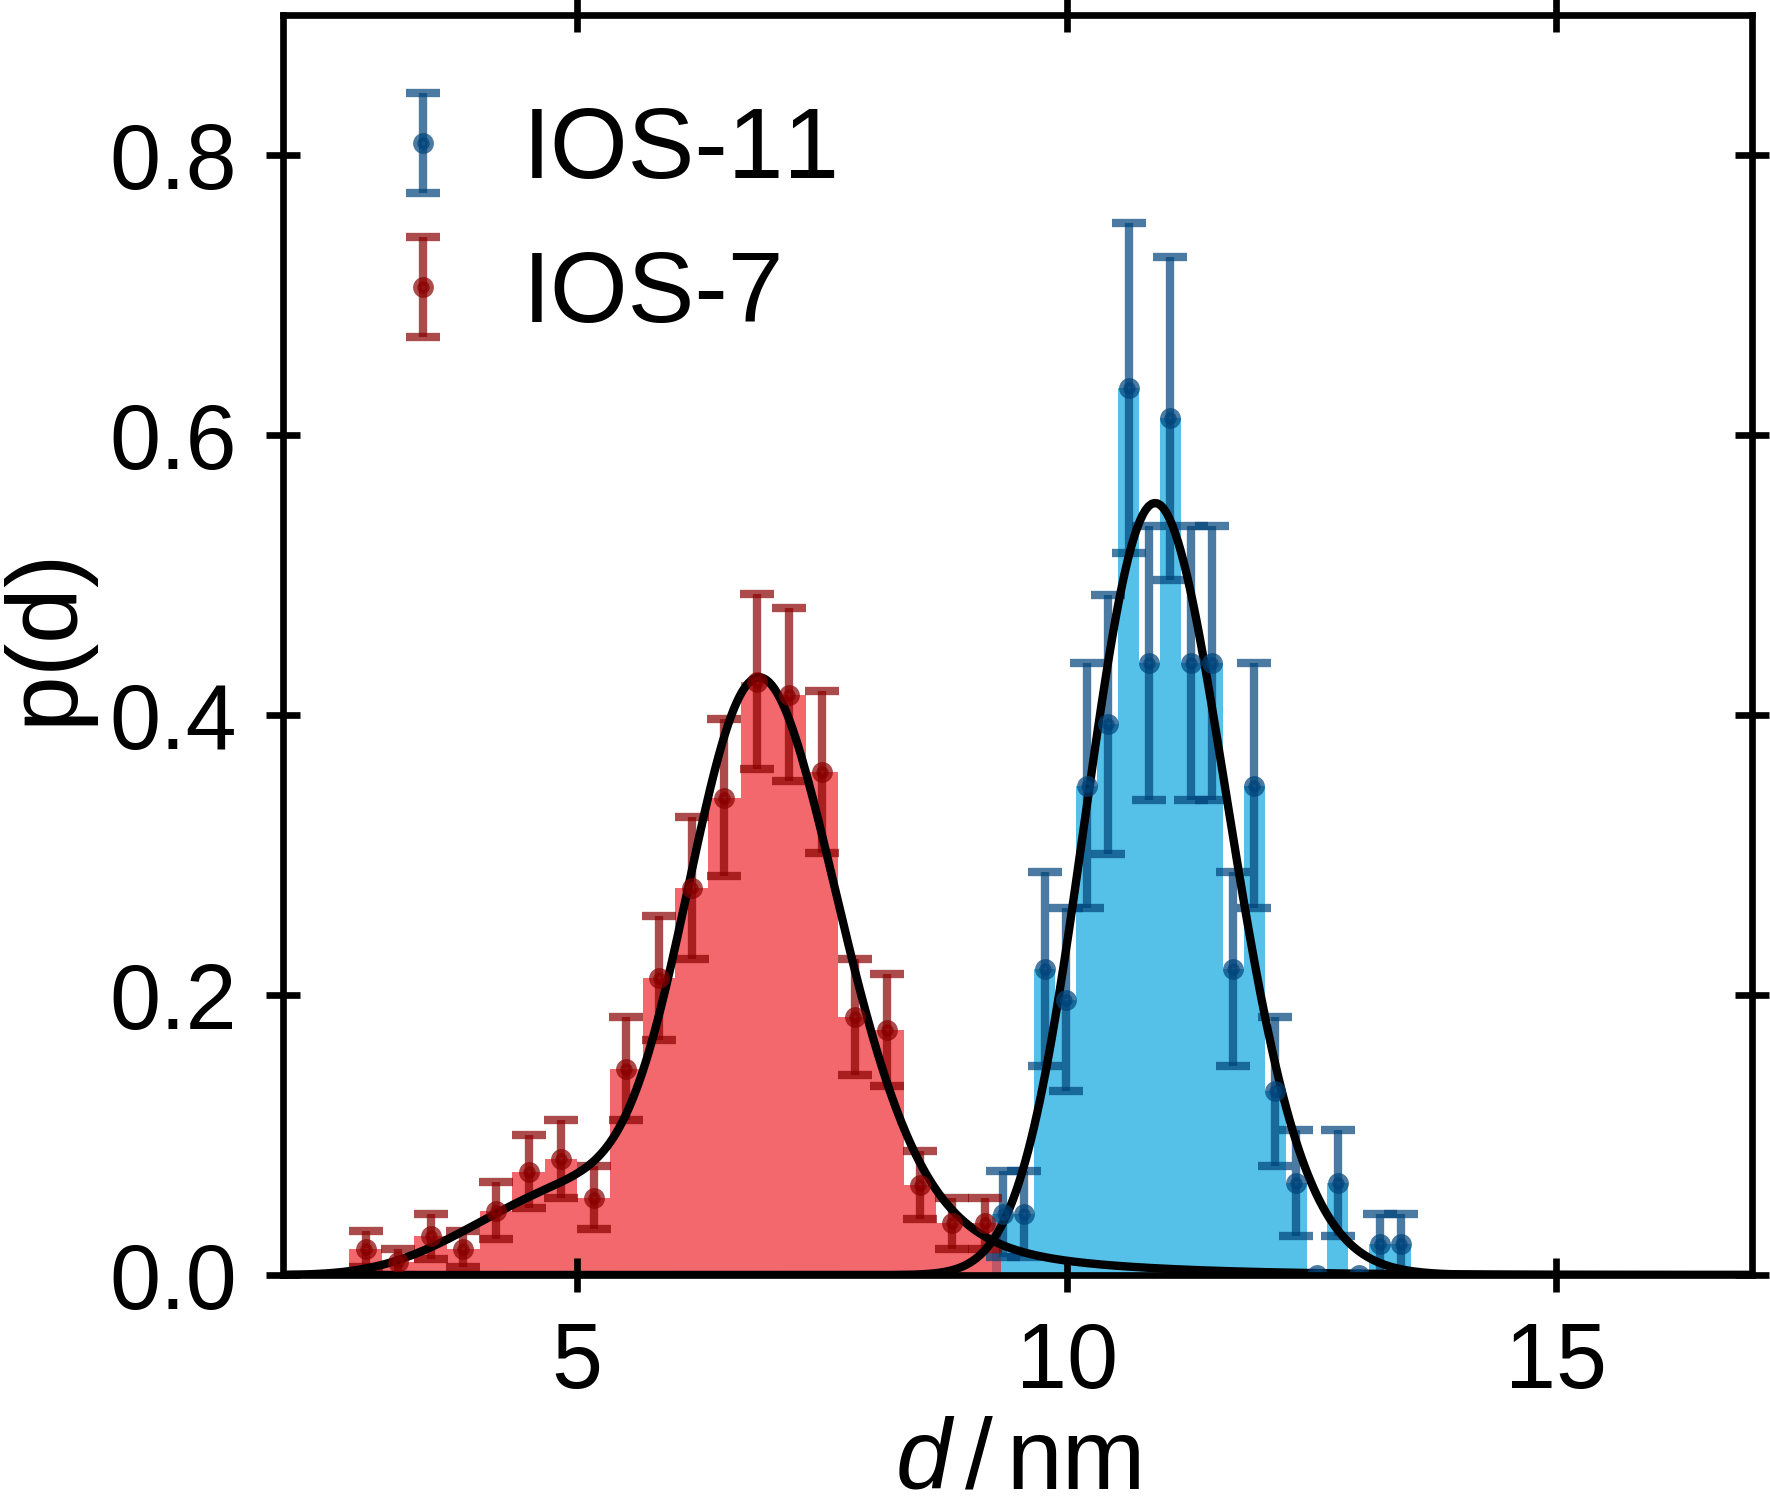
\includegraphics{looselyPackedNP_TEM_PMK18_KWi338_sizeDist}
    \caption{\label{fig:looselyPackedNP:nanoparticle:tem}TEM micrographs of iron oxide nanospheres IOS-11 (upper left) and IOS-7 (upper right), as well as the particle size distribution for the diameter for both samples (bottom).}
  \end{figure}

  Exemplarly micrographs of the two iron oxide nanosphere batches and the histograms of the counted occurence of diameters are shown in \reffig{fig:looselyPackedNP:nanoparticle:tem}.
  The spherical shape can be confirmed for both batches, where IOS-11 qualitatively shows a greater size and smaller size distribution in direct comparison to IOS-7.
  The different size is confirmed in the histograms and the fit to log-normal size distributions, where IOS-11 has a mean diameter of $10.95(5) \unit{nm}$ with a distribution of $6.6(4) \%$ and IOS-7 $6.97(6) \unit{nm}$ with $11(1) \%$.
  Due to the large size distribution of IOS-7, a bimodal distribution is fit in this case, where the second mode of nanoparticles has a mean diameter of $6.0(6) \unit{nm}$ and a distribution of $29(4) \%$.
  The fraction of the mode with the broad size distribution is estimated to be $30(10) \%$ of the sample.

  \begin{table}[!htbp]
    \centering
    \caption{\label{tab:looselyPackedNP:nanoparticle:temModel}Parameters estimated for the size distribution of IOS-11 and IOS-7 from fitting a (bimodal) log-normal size distribution.}
    \begin{tabular}{ c | l | l }
        & IOS-11 & IOS-7 \\
      \hline
      $\alpha$    & $1$                   & $0.7(1)$   \\
      $\mu_1$     & $10.95(5) \unit{nm}$  & $6.97(6) \unit{nm}$ \\
      $\sigma_1$  & $6.6(4) \unit{\%}$    & $11(1) \unit{\%}$ \\
      $\mu_2$     & -                     & $6.0(6) \unit{nm}$ \\
      $\sigma_2$  & -                     & $29(4) \unit{\%}$ \\
      \hline
    \end{tabular}
  \end{table}
\end{document}